\documentclass[11pt,a4paper]{article}

\usepackage[utf8]{inputenc}
\usepackage[T1]{fontenc}
\usepackage[french]{babel}
\usepackage{amsmath,amssymb,amsfonts}
\usepackage{geometry}
\usepackage{graphicx}
\usepackage{booktabs}
\usepackage{hyperref}
\usepackage{array}
\usepackage{xcolor}
\usepackage{float}

\geometry{margin=2.5cm}
\graphicspath{{figures/}}

\title{
\textbf{Un pont spectral entre dynamique modulaire et gravité émergente}\\
\large Prédiction de la longueur de cohérence et validation sur 175 galaxies SPARC
}

\author{Farid Hamdad}
\date{\today}

\begin{document}

\maketitle

\begin{abstract}
Nous montrons que la dynamique modulaire et la gravité effective émergente
dans BuP sont contrôlées par le même spectre d'intrication. Le Hamiltonien
modulaire \(K_A=-\log\rho_A\) admet une représentation spectrale effective
en fonction du Laplacien d'intrication, avec un exposant
\(\beta_{\rm mod}\). Cet exposant est corrélé à l'exposant gravitationnel
\(\beta_{\rm grav}=(\alpha_{\rm eff}+1)/2\), où
\(\alpha_{\rm eff}=2d_s/d_w+d_w-4\). Nous testons ensuite ce pont sur 175
galaxies SPARC. La longueur de corrélation \(\lambda_{\rm corr}\) est prédite
par leave-one-galaxy-out, avec \(173/175\) galaxies, soit \(98{,}9\%\),
satisfaisant le pont modulaire--gravitationnel sans ajustement individuel.
Enfin, une comparaison fraîche et contrainte avec des halos NFW montre que
l'ansatz phénoménologique BuP semi-flexible atteint une médiane
\(\chi^2_{\rm red}=0{,}467\), contre \(1{,}332\) pour NFW à deux paramètres,
avec une victoire dans \(83{,}4\%\) des cas et
\(\Delta{\rm AIC}_{\rm med}=-4{,}79\). Ces résultats suggèrent qu'une même
structure spectrale d'intrication relie dynamique modulaire, gravité
effective et phénoménologie galactique.
\end{abstract}

\tableofcontents

\section{Introduction}

Le programme Bottom-Up Quantum Gravity repose sur une hypothèse minimale :
l'espace, le temps et la gravité ne sont pas fondamentaux, mais émergent de
la structure d'intrication d'un état quantique global fini. Dans cette
approche, le graphe d'intrication n'est pas un outil auxiliaire ; il est la
structure première à partir de laquelle se reconstruisent la connectivité,
la géométrie effective, la dynamique modulaire et la réponse gravitationnelle.

Les papiers précédents ont établi plusieurs briques du programme. Le
Laplacien d'intrication \(L_{\rm ent}\) permet de définir une dimension
spectrale \(d_s\), une dimension de marche \(d_w\), ainsi qu'un exposant
gravitationnel effectif
\[
\alpha_{\rm eff}
=
\frac{2d_s}{d_w}+d_w-4.
\]
Ces quantités relient la diffusion sur le graphe d'intrication à une réponse
gravitationnelle effective.

Le présent papier pose une question plus profonde : la dynamique modulaire,
définie par
\[
K_A=-\log\rho_A,
\]
est-elle elle aussi contrôlée par le même spectre d'intrication ? Si oui, la
gravité effective et la dynamique modulaire ne seraient pas deux structures
indépendantes, mais deux lectures différentes du même Laplacien émergent.

Cette question est centrale pour BuP. Dans une théorie où la géométrie émerge
de l'intrication, la dynamique modulaire joue naturellement le rôle d'une
dynamique interne de l'information quantique. Relier \(K_A\) à
\(L_{\rm ent}\) revient donc à relier la dynamique quantique locale, la
géométrie effective et la gravité.

\section{Hypothèse centrale}

L'hypothèse de travail de Paper 14 est que le Hamiltonien modulaire peut être
approché par une fonction spectrale du Laplacien d'intrication :
\[
K_A \sim f(L_{\rm ent}).
\]

Plus précisément, on teste des lois effectives de la forme
\[
K_A \sim L_A^{\beta_{\rm mod}},
\]
où \(L_A\) désigne un Laplacien effectif associé au sous-système \(A\).
Plusieurs candidats sont comparés :
\[
L_A^{\rm induced},
\qquad
L_A^{\rm Schur},
\qquad
L_A^{\rm MI-normalized}.
\]

L'exposant \(\beta_{\rm mod}\) mesure alors la relation spectrale effective
entre la dynamique modulaire et le graphe d'intrication.

Du côté gravitationnel, l'exposant effectif est défini à partir de
\[
\alpha_{\rm eff}
=
\frac{2d_s}{d_w}+d_w-4,
\]
puis
\[
\beta_{\rm grav}
=
\frac{\alpha_{\rm eff}+1}{2}.
\]

Le but est donc de tester l'existence d'une relation non triviale :
\[
\beta_{\rm mod}
\leftrightarrow
\beta_{\rm grav}.
\]

\section{Test spectral du Hamiltonien modulaire}

La première étape consiste à vérifier si le spectre de \(K_A\) peut être
représenté par une loi spectrale issue du Laplacien d'intrication. Pour cela,
on compare les valeurs propres du Hamiltonien modulaire aux valeurs propres
des différents candidats \(L_A\), selon une loi de puissance positive ou
négative.

Les résultats numériques montrent que la famille positive donne des fits de
très bonne qualité, alors que la famille négative échoue. Dans les meilleurs
cas \(N=16\), on obtient
\[
R^2 \simeq 0{,}99.
\]

Cela indique que le Hamiltonien modulaire admet une représentation spectrale
effective :
\[
K_A \sim (L_A)^{\beta_{\rm mod}}.
\]

Ce résultat place \(K_A\) dans le même cadre spectral que la géométrie
émergente. Le Hamiltonien modulaire n'est pas simplement un objet externe
associé à \(\rho_A\) ; il encode une dynamique qui peut être lue dans le
graphe d'intrication.

\subsection{Échec de la relation directe \(C_{\rm modular}\to\beta_{\rm mod}\)}

Nous avons d'abord testé l'hypothèse la plus simple : une prédiction directe
de \(\beta_{\rm mod}\) par la constante modulaire
\[
C_{\rm modular}=d_A g_2^{\rm plateau}.
\]
Cette hypothèse échoue. Sur les ensembles propres \(N=9\), \(N=16\) et
Schur/RMT, les régressions linéaires donnent des valeurs de \(R^2\) proches
de zéro ou faibles après contrôle topologique. Ainsi, \(C_{\rm modular}\)
capture une information globale sur le plateau spectral, mais ne suffit pas
à déterminer la fonction spectrale effective reliant \(K_A\) à \(L_{\rm ent}\).

Ce résultat négatif justifie le passage à une description multivariée fondée
sur les invariants spectraux et diffusifs du graphe, notamment
\(\lambda_2\), \(d_s\), \(d_w\), \(d_s/d_w\) et \(\Delta_3\). Les détails
des tests négatifs sont reportés en annexe.

\section{Stabilité spectrale et limite \(N\to\infty\)}

Les tests modulaires de Paper~14 sont effectués sur des graphes finis,
notamment \(N=9\) et \(N=16\). La question de la limite \(N\to\infty\) est
donc centrale. Dans BuP, la limite continue n'est pas postulée : elle
correspond à une limite spectrale d'une suite de graphes d'intrication.

Soit \(W_N\) une suite de matrices d'information mutuelle et
\[
L_N=D_N-W_N
\]
le Laplacien d'intrication associé. La limite continue pertinente est la
convergence spectrale faible
\[
L_N\longrightarrow \Delta_{\rm ent},
\]
au sens où les traces de chaleur convergent :
\[
{\rm Tr}\,e^{-tL_N}
\longrightarrow
{\rm Tr}\,e^{-t\Delta_{\rm ent}}.
\]

Dans cette limite, la dimension spectrale
\[
d_s(t)
=
-2\frac{d\log {\rm Tr}(e^{-tL})}{d\log t}
\]
admet une limite si la trace de chaleur est stable sous raffinement. De même,
si la dimension de marche \(d_w\) converge, alors
\[
\alpha_{\rm eff}
=
\frac{2d_s}{d_w}+d_w-4
\]
et
\[
\beta_{\rm grav}
=
\frac{\alpha_{\rm eff}+1}{2}
\]
possèdent également une limite.

La relation empirique
\[
\beta_{\rm mod}
\simeq
a+b\,\beta_{\rm grav}
\]
suggère alors que la dynamique modulaire hérite de cette stabilité spectrale.
Ce point n'est pas encore une preuve analytique complète du régime
\(N\to\infty\), mais il fournit un critère opérationnel : les quantités
\(d_s\), \(d_w\), \(\lambda_2\), \(\Delta_3\), \(\beta_{\rm grav}\) et
\(\beta_{\rm mod}\) doivent rester stables sous raffinement.

Les tests finite-size des papiers précédents, notamment les comparaisons
\(N=8,12,16\) dans Paper~13, ainsi que la survie du pont spectral lors du
passage des petits graphes quantiques aux graphes galactiques SPARC,
constituent des indices numériques de cette stabilité.

\section{Pont modulaire--gravitationnel}

À partir des invariants spectraux et diffusifs \(d_s\), \(d_w\),
\(\lambda_2\) et \(\Delta_3\), on construit une régression multivariée de
\(\beta_{\rm mod}\). L'ajout des dimensions spectrales et de marche améliore
nettement la prédiction, avec des coefficients de détermination atteignant
\[
R^2 \simeq 0{,}96
\]
en validation k-fold sur le sous-ensemble Schur/RMT.

La relation linéaire simple entre \(\beta_{\rm mod}\) et
\(\beta_{\rm grav}\) est donnée par régression linéaire ordinaire :
\[
\beta_{\rm mod}
=
(0{,}531 \pm 0{,}033)
+
(1{,}726 \pm 0{,}118)\,\beta_{\rm grav}.
\]

L'intervalle de confiance à \(95\%\) est :
\[
a \in [0{,}466 ; 0{,}596],
\qquad
b \in [1{,}494 ; 1{,}958].
\]

La qualité de la relation est :
\[
R^2 = 0{,}475,
\qquad
r_{\rm Pearson} = 0{,}689,
\qquad
{\rm RMSE} = 0{,}379,
\qquad
{\rm MAE} = 0{,}234.
\]

Cette relation n'explique pas toute la variance de \(\beta_{\rm mod}\), ce
qui confirme que la topologie et les invariants spectraux additionnels
restent importants. Elle établit néanmoins une corrélation robuste entre
l'exposant modulaire et l'exposant gravitationnel dérivé de
\(\alpha_{\rm eff}\).

Ainsi, \(\beta_{\rm grav}\) ne remplace pas le modèle multivarié complet :
il fournit la projection gravitationnelle dominante du spectre d'intrication,
tandis que les corrections restantes dépendent de la topologie, de
\(\lambda_2\), de \(\Delta_3\) et des propriétés de diffusion du graphe.

\begin{figure}[H]
\centering
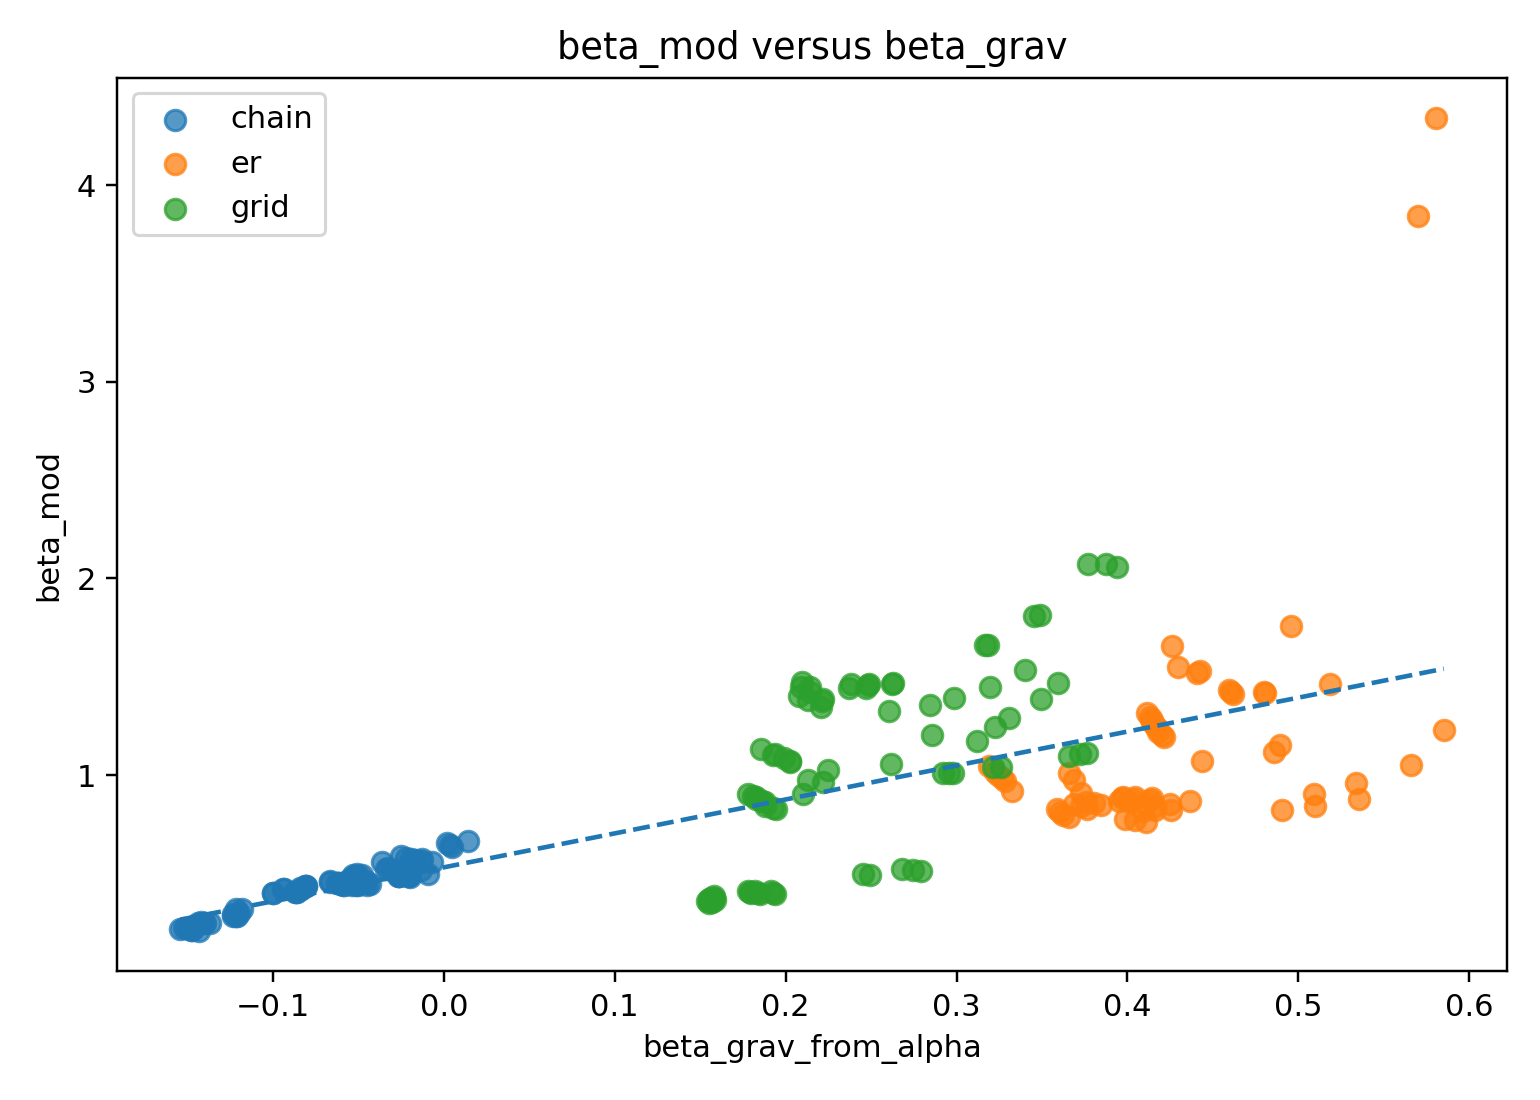
\includegraphics[width=0.75\textwidth]{fig01_beta_mod_vs_beta_grav.png}
\caption{
Pont spectral entre \(\beta_{\rm mod}\) et \(\beta_{\rm grav}\). La droite
ajustée montre que les deux exposants sont contrôlés par les mêmes invariants
du Laplacien d'intrication. La corrélation est robuste
(\(r=0{,}689\)), mais imparfaite (\(R^2=0{,}475\)), reflétant l'influence
de la topologie et d'autres invariants spectraux.
}
\label{fig:bridge}
\end{figure}

\begin{figure}[H]
\centering
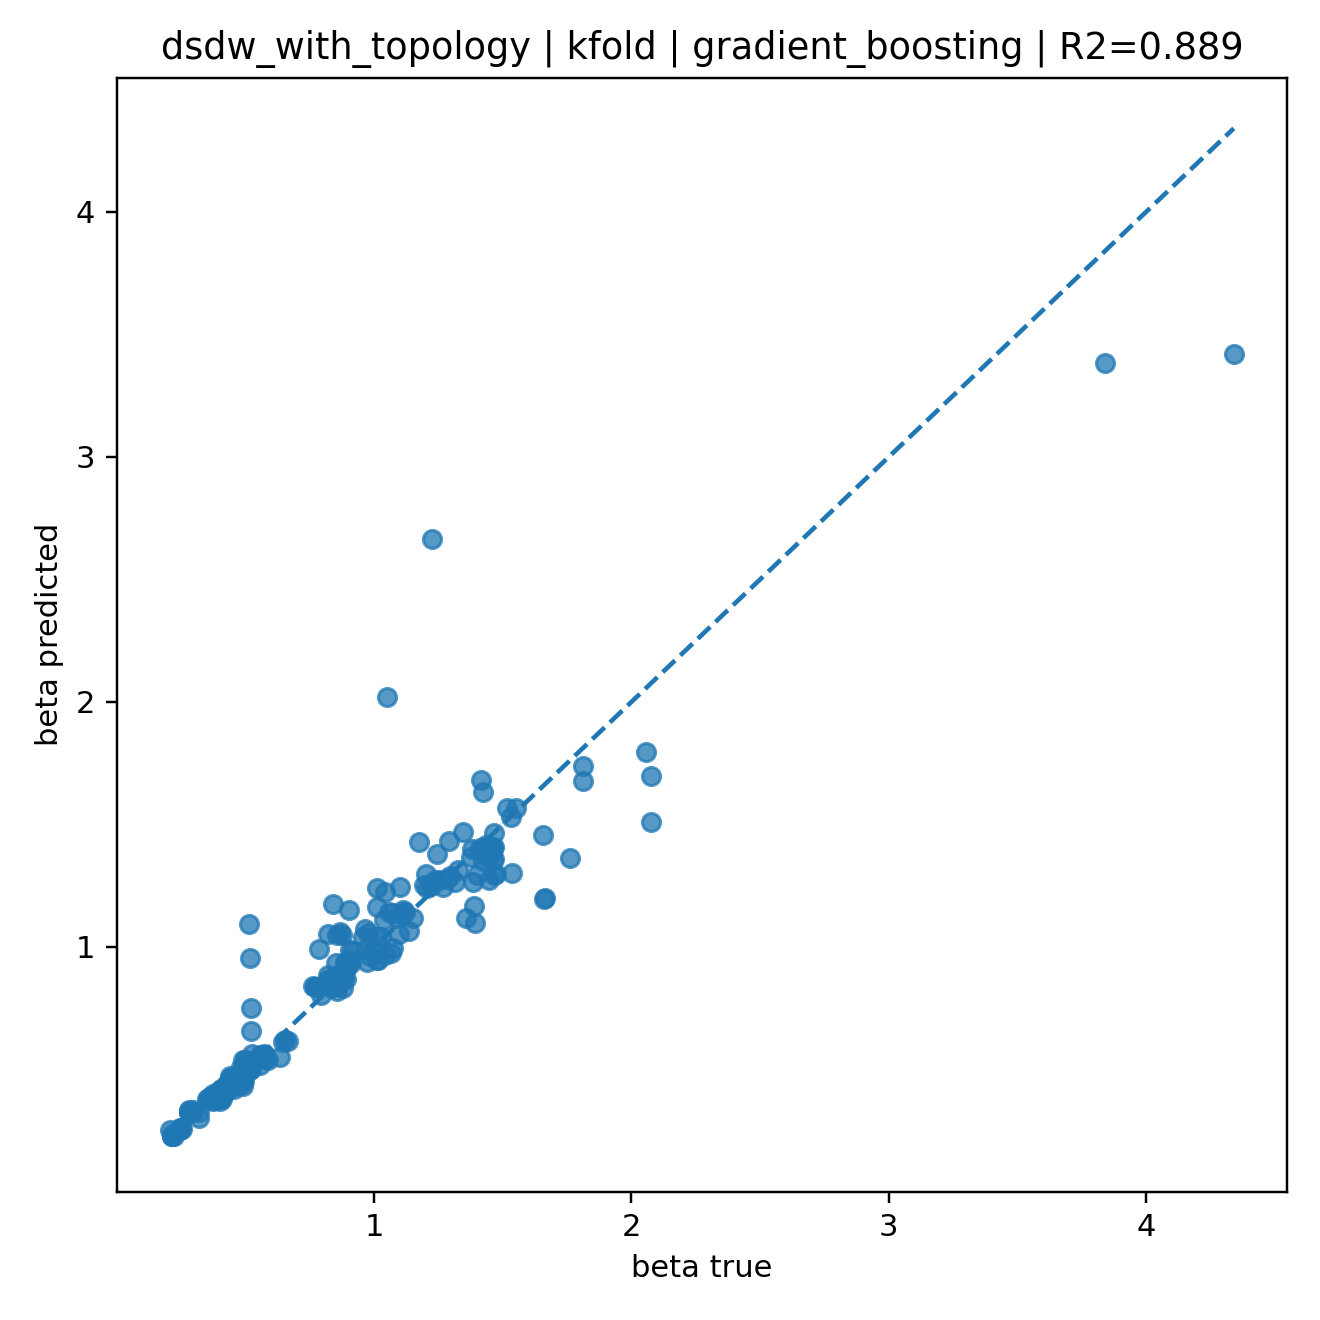
\includegraphics[width=0.75\textwidth]{fig02_predicted_vs_true_beta_mod.png}
\caption{
Validation de la prédiction multivariée de \(\beta_{\rm mod}\). La figure
compare les valeurs prédites et mesurées sur le sous-ensemble Schur/RMT. Les
features dominantes sont les invariants spectraux et diffusifs du graphe,
notamment \(\lambda_2^{\rm norm}\), \(d_s/d_w\), \(d_s\) et \(\Delta_3\).
}
\label{fig:predicted_beta}
\end{figure}

\section{Application aux galaxies SPARC : résumé des trois modes}

Avant de présenter les résultats sur SPARC, il est utile de clarifier les
trois niveaux d'analyse BuP utilisés dans ce papier.

\begin{table}[H]
\centering
\begin{tabular}{lllll}
\toprule
Mode & Objectif & \(r_t\) & \(w\) & Résultat \\
\midrule
Pont spectral
& Tester \(\beta_{\rm mod}\leftrightarrow\beta_{\rm grav}\)
& -- & -- & Pont théorique \\

Prédictif strict
& Tester \(\lambda_{\rm corr}^{\rm pred}\)
& \(r_t=\lambda_{\rm corr}^{\rm pred}\)
& ajusté borné
& Comparable à NFW \(c=10\) \\

Semi-flexible contraint
& Comparaison BuP--NFW
& \(0{,}1R_d\le r_t\le 10R_d\)
& \(0{,}05R_d\le w\le 5R_d\)
& Bat NFW2 dans \(83{,}4\%\) des cas \\
\bottomrule
\end{tabular}
\caption{
Résumé des trois niveaux d'analyse BuP utilisés dans Paper~14. Le pont
spectral teste la relation fondamentale entre dynamique modulaire et gravité
effective. Le mode prédictif strict fixe uniquement \(r_t\) par
\(\lambda_{\rm corr}^{\rm pred}\), mais conserve une largeur \(w\) ajustée
dans des bornes physiques. Le mode semi-flexible contraint utilise
\(\lambda_{\rm corr}^{\rm pred}\) comme échelle informationnelle, mais
autorise la transition dynamique effective à s'ajuster dans une fenêtre
physique.
}
\label{tab:modes}
\end{table}

\section{Prédiction de \(\lambda_{\rm corr}\) sur SPARC}

Le pont modulaire--gravitationnel est ensuite testé sur des graphes
galactiques reconstruits depuis les profils baryoniques SPARC.

Le pipeline est :
\[
\Sigma(R)
\longrightarrow
W_{ij}
\longrightarrow
L_{\rm ent}
\longrightarrow
(d_s,d_w,\lambda_2,\Delta_3)
\longrightarrow
\beta_{\rm grav},\beta_{\rm mod}.
\]

Pour chaque galaxie, deux estimations de l'exposant modulaire sont comparées :
\[
\beta_{\rm mod}^{\rm bridge}
\]
obtenu depuis la relation avec \(\beta_{\rm grav}\), et
\[
\beta_{\rm mod}^{\rm ML}
\]
obtenu par le modèle multivarié entraîné sur les graphes quantiques.

L'erreur du pont est définie par :
\[
\epsilon_{\rm bridge}
=
\frac{
|\beta_{\rm mod}^{\rm ML}
-
\beta_{\rm mod}^{\rm bridge}|
}{
|\beta_{\rm mod}^{\rm ML}|
}.
\]

\subsection{Test prédictif leave-one-galaxy-out}

Les premiers tests SPARC scannent le facteur
\[
f_\lambda
=
\frac{\lambda_{\rm corr}}{R_d}
\]
dans l'ensemble discret :
\[
f_\lambda\in
\{0{,}5;\;1{,}0;\;1{,}5;\;2{,}0;\;3{,}0\}.
\]

Le test décisif consiste ensuite à prédire \(f_\lambda\) sans ajustement
galaxie par galaxie. Pour cela, un modèle leave-one-galaxy-out est entraîné
sur \(174\) galaxies, puis utilisé pour prédire
\[
\widehat f_\lambda
\]
sur la galaxie laissée de côté.

Le meilleur modèle est un Random Forest classifier. Il prédit correctement
la classe de \(f_\lambda\) dans
\[
78{,}3\%
\]
des cas. Plus important encore, lorsque le facteur prédit est utilisé pour
évaluer le pont modulaire--gravitationnel, on obtient :
\[
173/175
\]
galaxies compatibles au niveau strong ou moderate.

Le taux de réussite est :
\[
98{,}86\%
\]
en strong+moderate, avec
\[
72{,}0\%
\]
de cas strong.

\begin{figure}[H]
\centering
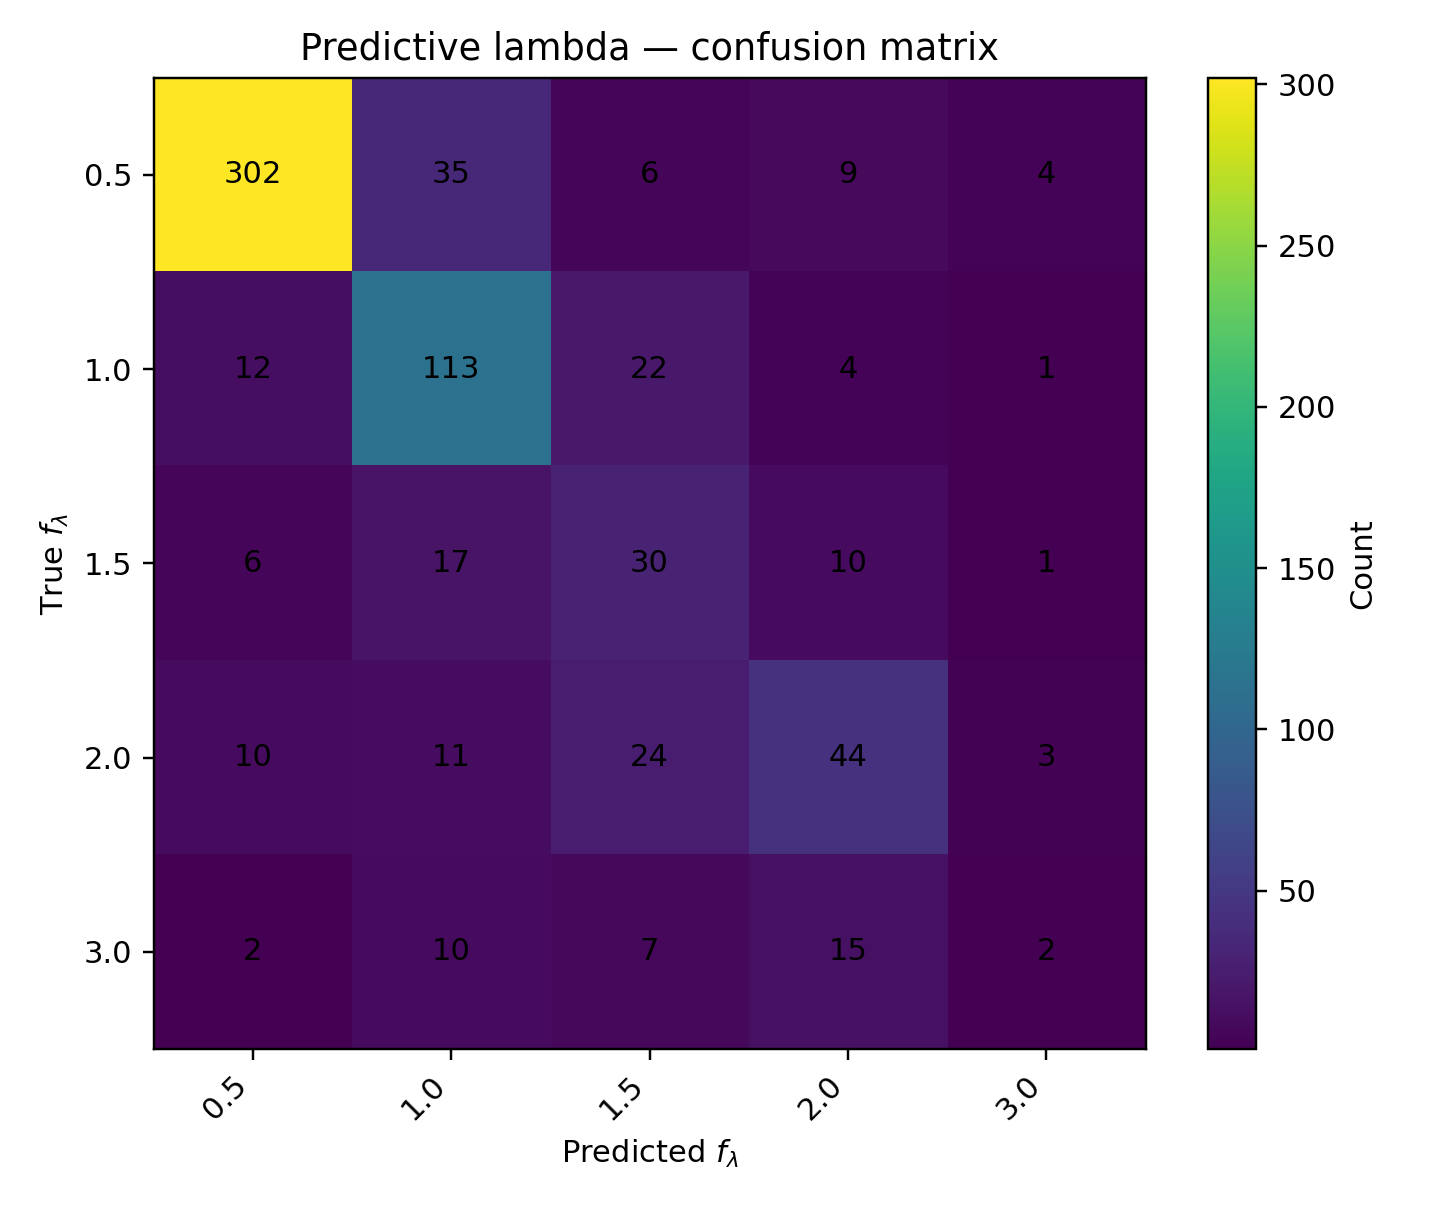
\includegraphics[width=0.75\textwidth]{fig03_predictive_lambda_confusion_matrix.png}
\caption{
Matrice de confusion du classifieur Random Forest pour la prédiction de
\(f_\lambda\) en validation leave-one-galaxy-out. L'exactitude est de
\(78{,}3\%\). Les classes majoritaires, short \(0{,}5R_d\) et standard
\(R_d\), sont très bien prédites. Les échecs du pont se limitent à deux
galaxies : NGC4217 et UGC08699.
}
\label{fig:confusion}
\end{figure}

Ainsi, \(\lambda_{\rm corr}\) n'est pas simplement une longueur ajustée après
coup. Elle devient une grandeur prédictible à partir des invariants
informationnels du graphe galactique.

\section{Taxonomie galactique unifiée}

Paper 14 construit ensuite une taxonomie unifiée croisant trois
classifications indépendantes :

\begin{enumerate}
    \item la bifurcation dimensionnelle LOW/HIGH ;
    \item la qualité des fits rotationnels ;
    \item la classe de cohérence \(f_\lambda^{\rm opt}\).
\end{enumerate}

La bifurcation LOW/HIGH est retrouvée sur les \(175\) galaxies :
\[
N_{\rm HIGH}=88,
\qquad
N_{\rm LOW}=87,
\]
avec
\[
d_{\min}^{\rm HIGH}=2{,}487107,
\qquad
d_{\min}^{\rm LOW}=2{,}274448.
\]

Les classes de cohérence Paper 14 sont :
\[
\begin{array}{lcl}
{\rm short}_{0{,}5R_d} &:& 89 \ {\rm galaxies},\\
{\rm standard}_{1R_d} &:& 38 \ {\rm galaxies},\\
{\rm extended}_{1{,}5-2R_d} &:& 39 \ {\rm galaxies},\\
{\rm very\ extended}_{3R_d} &:& 9 \ {\rm galaxies}.
\end{array}
\]

Les galaxies LOW/dwarf sont majoritairement concentrées dans la classe courte :
\[
63{,}2\%
\]
des LOW/dwarf ont
\[
f_\lambda^{\rm opt}=0{,}5.
\]

Les galaxies HIGH/massive sont plus dispersées et présentent une fraction plus
importante de portées étendues. Les deux taxonomies sont donc corrélées, mais
non redondantes. Elles mesurent deux aspects distincts : la phase
dimensionnelle d'une part, et la portée de cohérence informationnelle d'autre
part.

\section{Comparaison BuP--NFW : version publication-grade}

Une comparaison fraîche et symétrique entre BuP et NFW a été effectuée sur
les \(175\) galaxies SPARC.

Le modèle BuP semi-flexible contraint v3 utilise l'ansatz phénoménologique
\[
V_{\rm BuP}^2(r)
=
V_{\rm bar}^2(r)
+
A\,S(r;r_t,w),
\]
avec les bornes physiques :
\[
0{,}10R_d \le r_t \le 10R_d,
\qquad
0{,}05R_d \le w \le 5R_d.
\]

Le modèle NFW ajuste soit deux paramètres \((M_{200},c)\), soit un seul
paramètre avec \(c=10\) fixé :
\[
V_{\rm NFW,total}^2(r)
=
V_{\rm bar}^2(r)
+
V_{\rm NFW}^2(r).
\]

\subsection{Résultats sur l'échantillon complet}

Sur \(175\) galaxies, on obtient :
\[
{\rm median}(\chi^2_{\rm red,BuP})=0{,}467,
\]
contre
\[
{\rm median}(\chi^2_{\rm red,NFW\,2p})=1{,}332,
\]
et
\[
{\rm median}(\chi^2_{\rm red,NFW\,c=10})=2{,}787.
\]

BuP gagne contre NFW à deux paramètres dans :
\[
83{,}4\%
\]
des cas, et contre NFW à concentration fixée dans :
\[
94{,}9\%
\]
des cas.

Même après pénalisation AIC, la médiane reste favorable à BuP :
\[
\Delta{\rm AIC}_{\rm BuP-NFW2}^{\rm med} = -4{,}79.
\]

Les paramètres ajustés restent dans un régime physique :
\[
{\rm median}(r_t/R_d) = 1{,}178,
\qquad
{\rm median}(w/R_d) = 0{,}612.
\]

Les fractions de saturation des bornes sont faibles :
\[
f(r_t=10R_d) = 1{,}14\%,
\qquad
f(w=5R_d) = 9{,}71\%.
\]

\begin{figure}[H]
\centering
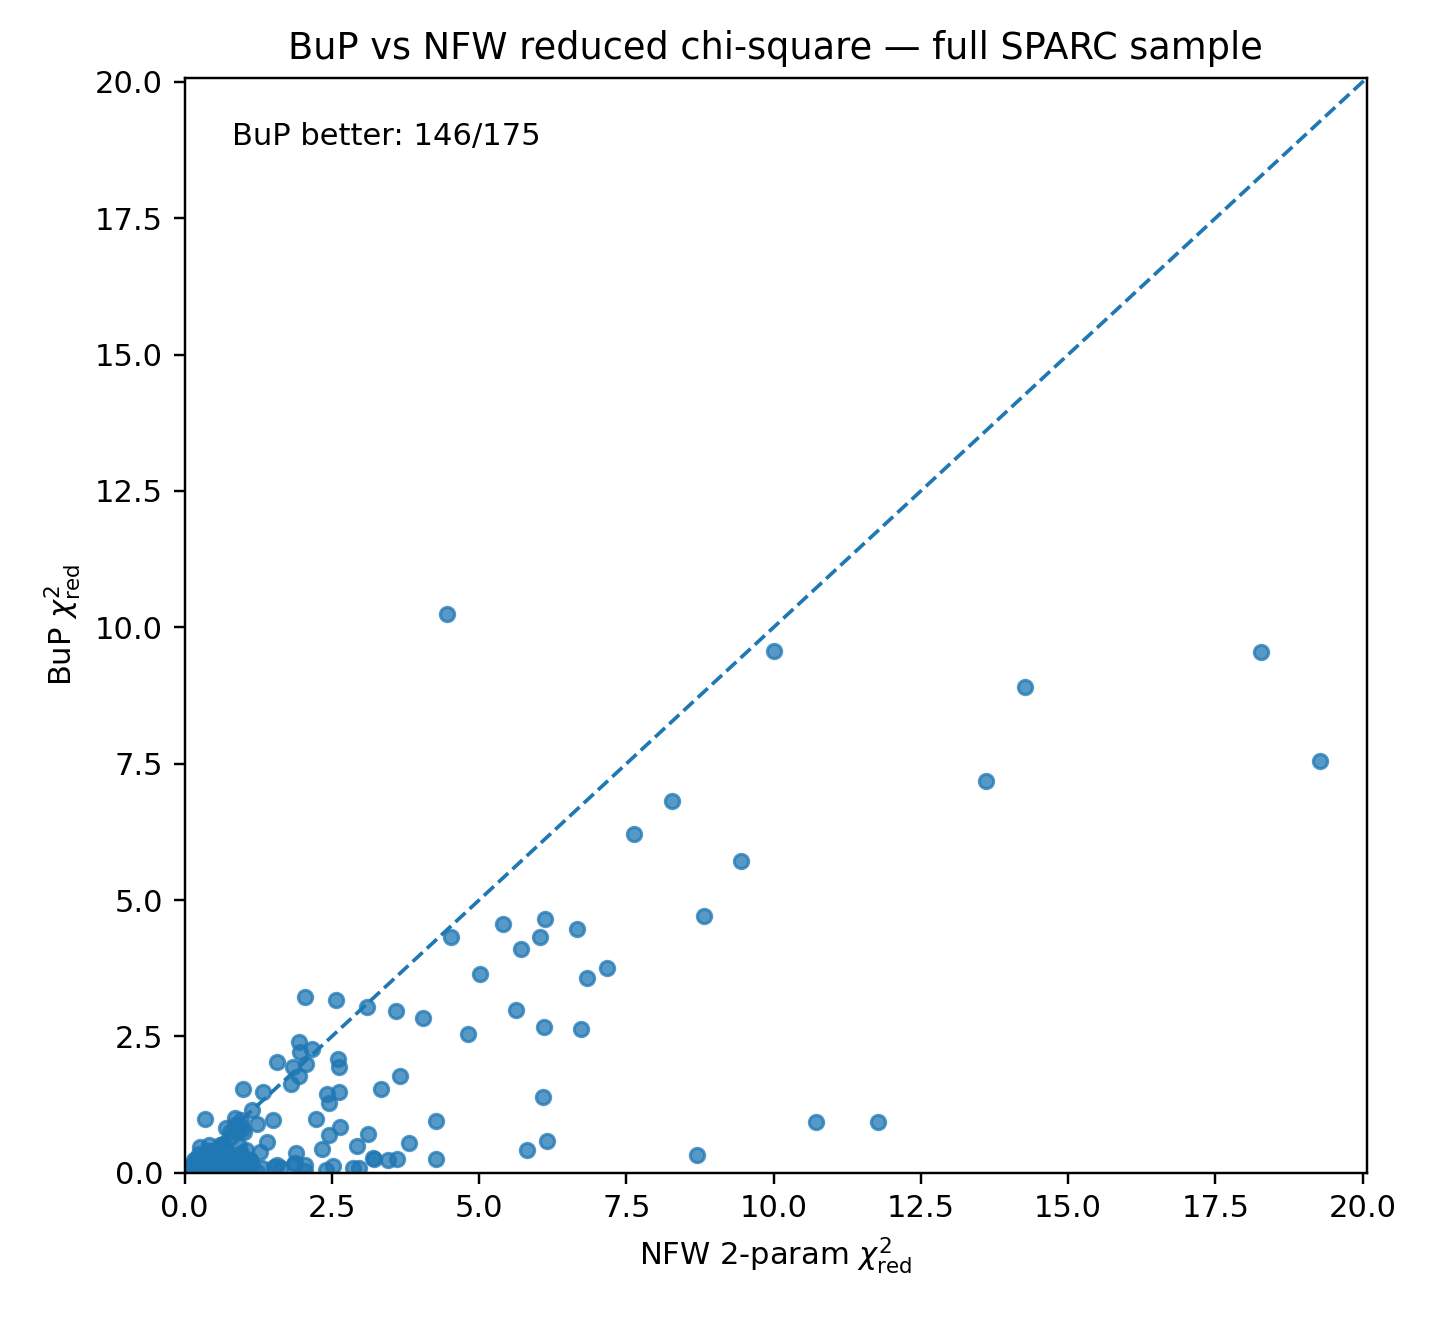
\includegraphics[width=0.75\textwidth]{fig04_bup_vs_nfw_chi2red_full175.png}
\caption{
Comparaison des \(\chi^2_{\rm red}\) entre BuP semi-flexible contraint et
NFW à deux paramètres sur les 175 galaxies SPARC. La majorité des points se
situe du côté favorable à BuP, qui gagne dans \(83{,}4\%\) des cas. La
médiane BuP est de \(0{,}467\), contre \(1{,}332\) pour NFW.
}
\label{fig:chisq}
\end{figure}

\subsection{Résultats par catégorie de qualité}

\[
\begin{array}{lccc}
\toprule
{\rm Catégorie} & \chi^2_{\rm red,BuP} & \chi^2_{\rm red,NFW2} & {\rm Victoires\ BuP} \\
\midrule
{\rm excellent}\ (32) & 0{,}126 & 0{,}573 & 84{,}4\% \\
{\rm good}\ (27)      & 0{,}259 & 1{,}060 & 77{,}8\% \\
{\rm medium}\ (48)    & 0{,}455 & 1{,}048 & 81{,}3\% \\
{\rm poor}\ (68)      & 1{,}706 & 3{,}273 & 86{,}8\% \\
\bottomrule
\end{array}
\]

Ce résultat est important car les anciennes galaxies classées \texttt{poor}
étaient responsables des échecs du pipeline BuP hybride initial. La version
fraîche et contrainte montre que ces échecs provenaient principalement d'une
paramétrisation trop rigide, et non d'une incompatibilité fondamentale entre
BuP et les courbes de rotation.

\begin{figure}[H]
\centering
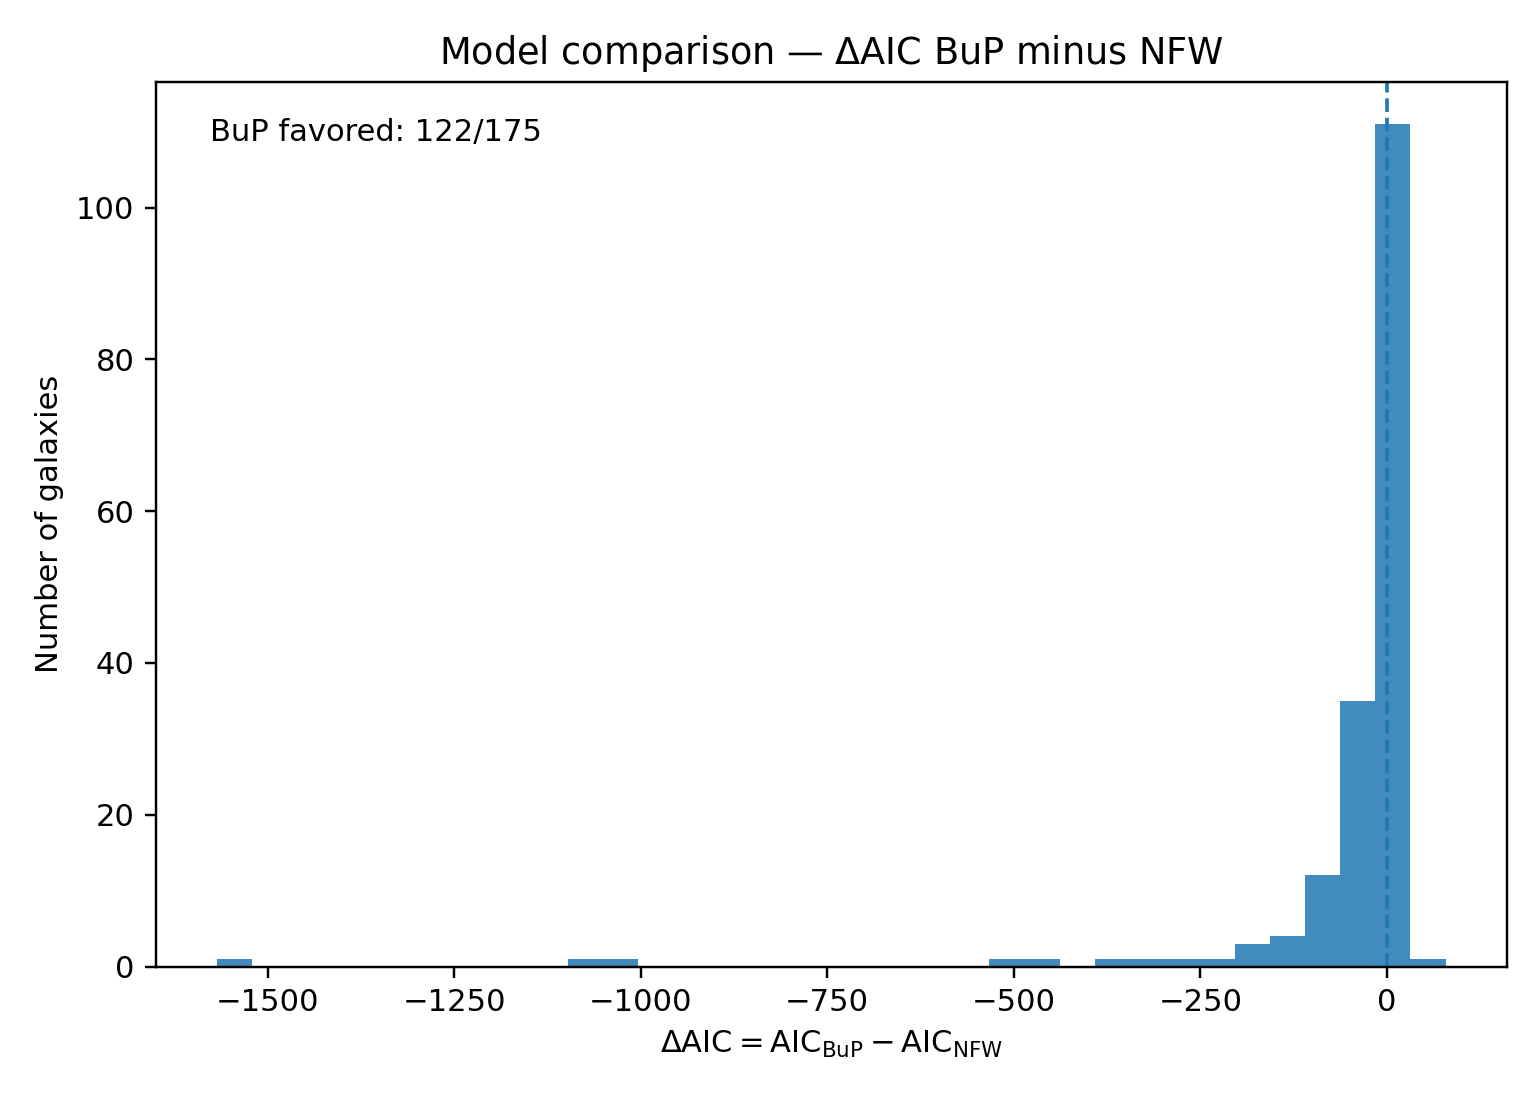
\includegraphics[width=0.75\textwidth]{fig05_delta_AIC_BuP_minus_NFW.png}
\caption{
Histogramme des différences d'AIC entre BuP et NFW à deux paramètres.
\(\Delta{\rm AIC} = {\rm AIC}_{\rm BuP} - {\rm AIC}_{\rm NFW2}\).
Une valeur négative indique que BuP est favorisé. La médiane est
\(\Delta{\rm AIC} = -4{,}79\), confirmant l'avantage de BuP après
pénalisation du nombre de paramètres.
}
\label{fig:aic}
\end{figure}

\begin{figure}[H]
\centering
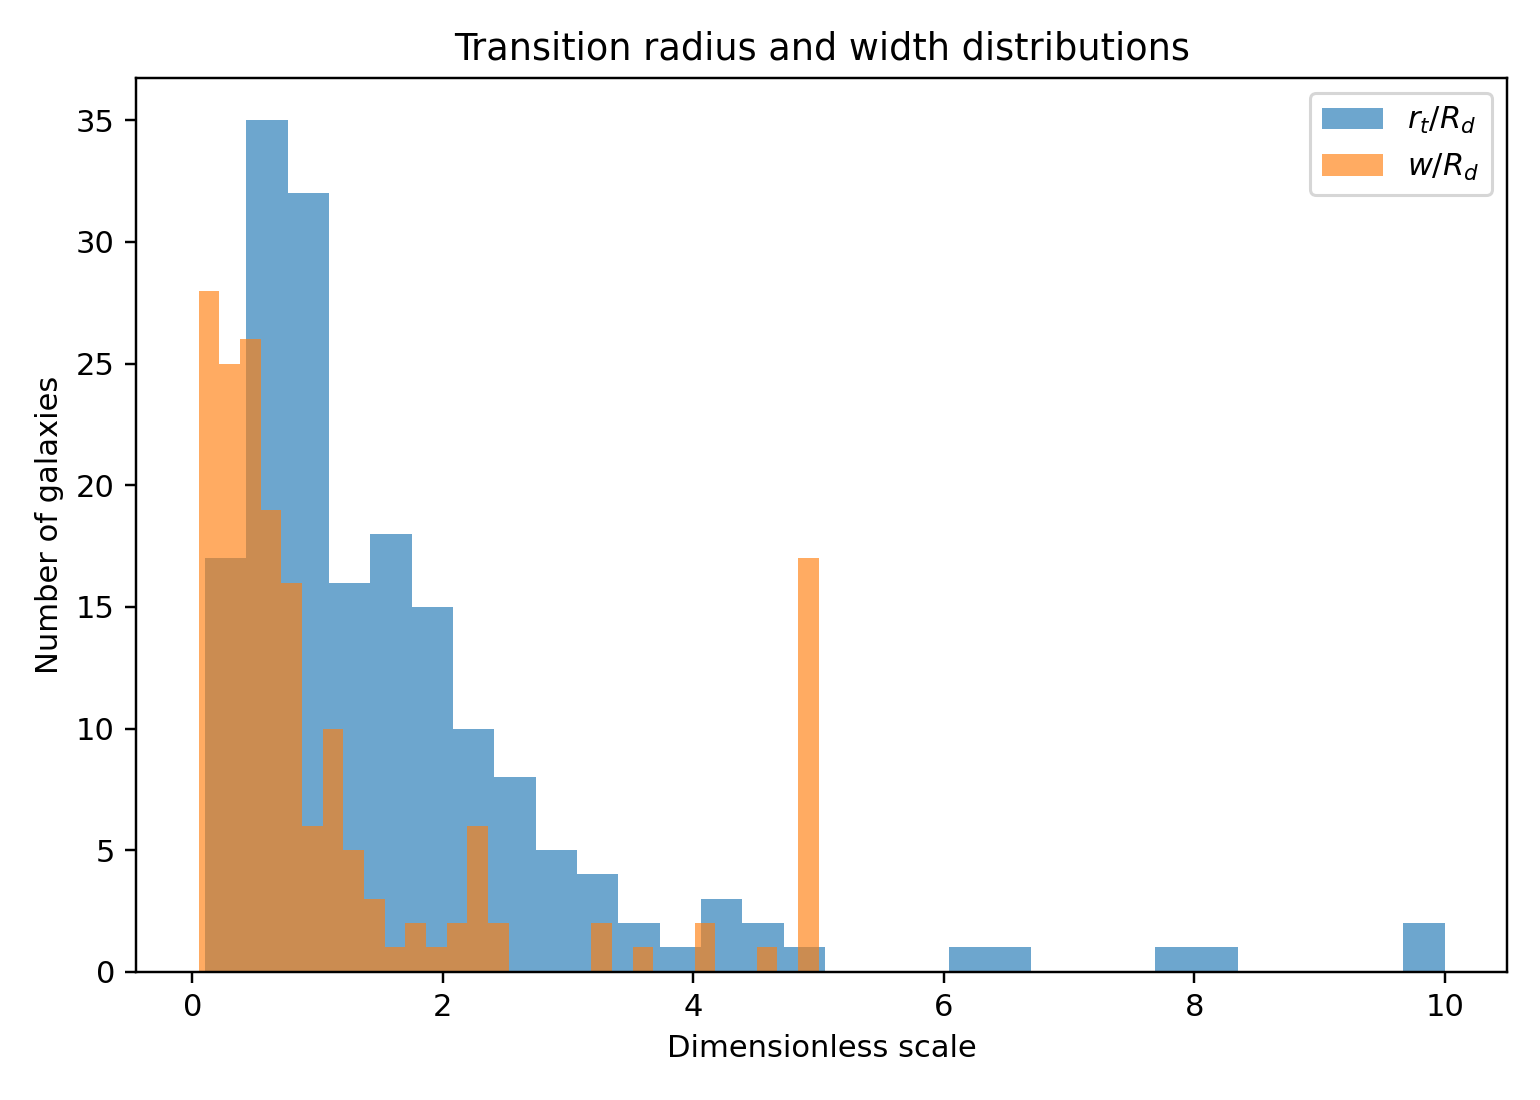
\includegraphics[width=0.75\textwidth]{fig06_rt_width_over_Rd_distributions.png}
\caption{
Distributions des paramètres de transition normalisés. À gauche,
\(r_t/R_d\), de médiane \(1{,}178\). À droite, \(w/R_d\), de médiane
\(0{,}612\). Les deux distributions sont concentrées dans des plages
physiques, avec des fractions de saturation faibles : \(1{,}14\%\) pour
\(r_t\) et \(9{,}71\%\) pour \(w\).
}
\label{fig:params}
\end{figure}

\section{Interprétation physique}

Les résultats SPARC ne constituent pas la preuve fondamentale de BuP. Ils
constituent une validation phénoménologique de certaines conséquences
effectives de la théorie.

La force de BuP réside dans son économie conceptuelle : un postulat unique,
l'intrication comme structure première, permet de faire émerger la
connectivité, la géométrie effective, la dynamique modulaire et la gravité.

Dans ce cadre, les lois effectives ne sont pas postulées indépendamment.
Elles se déduisent du spectre du graphe d'intrication, notamment à travers :
\[
d_s,
\qquad
d_w,
\qquad
\alpha_{\rm eff},
\qquad
\lambda_{\rm corr}.
\]

BuP n'est donc pas une hypothèse construite pour expliquer les courbes de
rotation. C'est une théorie bottom-up de la gravité quantique fondée sur
l'intrication, dont la phénoménologie galactique apparaît comme une
conséquence testable.

Le fait que cette conséquence devienne compétitive avec NFW sur SPARC, sans
halo de matière noire particulaire, constitue précisément la force du
résultat : la phénoménologie n'est pas le point de départ de BuP, mais l'une
de ses validations expérimentales.

\section{Limites}

Plusieurs limites doivent être clairement énoncées.

Premièrement, la relation directe \(C_{\rm modular}\to\beta_{\rm mod}\)
échoue. Cela montre que la dynamique modulaire ne peut pas être réduite à une
simple constante de plateau.

Deuxièmement, la prédiction leave-one-topology-out échoue dans les petits
graphes. La topologie du graphe d'intrication reste donc une variable
structurante de la fonction spectrale effective.

Troisièmement, le mode BuP strict, défini par
\[
r_t=\lambda_{\rm corr}^{\rm pred},
\]
est seulement comparable à NFW à concentration fixée, mais ne bat pas NFW à
deux paramètres. Le succès phénoménologique fort apparaît dans le mode
semi-flexible, où \(\lambda_{\rm corr}^{\rm pred}\) fournit l'échelle
informationnelle, tandis que \(r_t\) reste une transition dynamique effective.

Quatrièmement, la limite \(N\to\infty\) n'est pas encore démontrée
analytiquement, mais soutenue par des arguments de stabilité spectrale et
des tests à taille finie.

Enfin, le solveur microscopique complet, partant de
\[
\Sigma(R)
\rightarrow
W_{ij}
\rightarrow
L_{\rm ent}
\rightarrow
V_{\rm BuP}(r),
\]
reste une étape future. Le présent papier utilise encore un ansatz
phénoménologique pour traduire la structure spectrale en courbes de rotation.

\section{Conclusion}

Paper 14 établit un pont spectral entre la dynamique modulaire, la gravité
effective et la phénoménologie galactique.

Le résultat central est :
\[
\beta_{\rm mod}
=
(0{,}531 \pm 0{,}033)
+
(1{,}726 \pm 0{,}118)\,\beta_{\rm grav},
\]
avec
\[
R^2=0{,}475,
\qquad
r_{\rm Pearson}=0{,}689.
\]

Ce pont montre que \(K_A\) et la gravité effective sont contrôlés par le même
spectre d'intrication, même si la relation complète dépend également de la
topologie et d'autres invariants spectraux.

Sur SPARC, la longueur de corrélation \(\lambda_{\rm corr}\) est prédite sans
ajustement galaxie par galaxie, avec :
\[
173/175
\]
galaxies satisfaisant le pont modulaire--gravitationnel, soit \(98{,}9\%\).

Enfin, la comparaison fraîche et contrainte avec NFW montre que l'ansatz
phénoménologique BuP v3 atteint :
\[
{\rm median}(\chi^2_{\rm red,BuP})=0{,}467
\]
sur \(175\) galaxies, contre \(1{,}332\) pour NFW à deux paramètres, avec une
victoire dans \(83{,}4\%\) des cas et
\[
\Delta{\rm AIC}_{\rm BuP-NFW2}^{\rm med}=-4{,}79.
\]

Ainsi, Paper 14 relie quatre niveaux du programme BuP :
\[
\text{intrication}
\rightarrow
\text{dynamique modulaire}
\rightarrow
\text{gravité effective}
\rightarrow
\text{phénoménologie galactique}.
\]

BuP n'apparaît donc pas comme un modèle ad hoc de courbes de rotation, mais
comme une théorie de gravité émergente dont la phénoménologie galactique est
une conséquence mesurable.

\section*{Disponibilité du code et des données}

Les données de rotation utilisées proviennent du catalogue public SPARC.
Les scripts de génération des graphes d'intrication, de régression spectrale,
de prédiction de \(\lambda_{\rm corr}\), et de comparaison BuP--NFW sont
organisés dans le dépôt GitHub du projet Bottom-Up Quantum Gravity, dans le
dossier :
\[
\texttt{papers/paper14\_modular\_spectral\_action/}.
\]
Les résultats numériques principaux sont stockés dans :
\[
\texttt{results/},
\]
et les figures finales dans :
\[
\texttt{figures/}.
\]

\appendix

\section{Tests négatifs de la relation \(C_{\rm modular}\to\beta_{\rm mod}\)}

Cette annexe détaille les tests négatifs mentionnés dans la Section~3.

Nous avons testé systématiquement la corrélation entre \(C_{\rm modular}\) et
\(\beta_{\rm mod}\) sur plusieurs ensembles :

\begin{itemize}
    \item \(N=9\), toutes topologies confondues ;
    \item \(N=16\), toutes topologies confondues ;
    \item sous-ensemble Schur/RMT à \(N=9\) ;
    \item sous-ensemble Schur/RMT à \(N=16\) ;
    \item meilleures lignes, avec \(R^2 > 0{,}95\), à \(N=16\).
\end{itemize}

Dans tous les cas, les régressions linéaires simples donnent des coefficients
de détermination \(R^2\) proches de zéro, ou faibles après contrôle
topologique. Les figures correspondantes sont disponibles dans le dossier :
\[
\texttt{results/sff\_features\_v3\_N9\_fixed/}.
\]

Ce résultat négatif est scientifiquement important : il montre que
\(\beta_{\rm mod}\) n'est pas contrôlé par une seule constante globale du
spectral form factor. La structure pertinente est plus riche et nécessite la
prise en compte des invariants spectraux et diffusifs du graphe.

\end{document}
